En este capítulo vamos a dar una introducción a las bases de datos tipo NoSQL, veremos los principales usos de estas así como comparativas con bases de datos de tipo SQL.

Terminaremos este capítulo viendo las características más relevantes de la base de datos Mongo DB, la que utilizaremos en nuestro trabajo para dar una propuesta de un motor difuso para consultas sobre esta plataforma.

\section{Introducción}
NoSQL - \texttt{Not only SLQ} - la primera ocurrencia del término  según \cite{chalmerthesis} data de 1998 cuando Carlo Strozzi lo utiliza para denominar a la base de datos que había creado, una base de datos "open-source" relacional, \cite{strozzidb}, pero que no proveía de una interfaz SQL. En ese mismo artículo, datan de 2009 cuando Eric Evan retoma el término en unas conferencia sobre bases de datos "open-source".

A pesar de estas fechas y momentos puntuales, lo cierto es que las bases de datos clave-valor, por ejemplo, ahora consideradas NoSQL, existen desde mucho antes, por lo que es difícil encontrar referencias 

Hay muchas diferencias entre las base de datos NoSQL y los SGBDR (Sistema de Gestión de Bases de Datos Relacionales), veremos más adelante algunas de ellas, pero podemos destacar 2: El no uso del lenguaje SQL como lenguaje principal de consulta y que no garantizan completamente ACID (atomicidad, consistencia, aislamiento y durabilidad). 

La utilidad de este tipo de bases de datos se ha incrementado recientemente por la necesidad de incrementar el almacenamiento de datos. Son las principales bases de datos para las técnicas de Big Data y el manejo de grandes cantidades de datos. Suelen escalar bien horizontalmente y permiten el almacenamientos de distintas formas, veremos los tipos de bases de datos y algunos ejemplos en la siguiente sección.

\subsection{Teorema de CAP}
Vamos a aprovechar el teorema de CAP para hacer una primera clasificación de bases de datos \cite{captheorem}.

El \textbf{teorema de CAP} nos dice que es imposible garantizar a la misma vez: consistencia, disponibilidad y tolerancia a particiones:

\textbf{Consistencia}: La información tiene que ser la misma para una operación independientemente del nodo en el que se haga.

\textbf{Disponibilidad}: La información tiene que estar accesible para todos los clientes independientemente de que algún nodo no esté disponible.

\textbf{Tolerancia a particiones}: El sistema tiene que seguir disponible aunque existan problemas de comunicación entre algunos nodos y provoque una partición del mismo.

En base a estas definiciones, la siguiente imagen nos proporciona una clasificación de algunas de las bases de datos más utilizadas en función de las 2 características elegidas para su definición.

\begin{figure}[h]
  \centering
  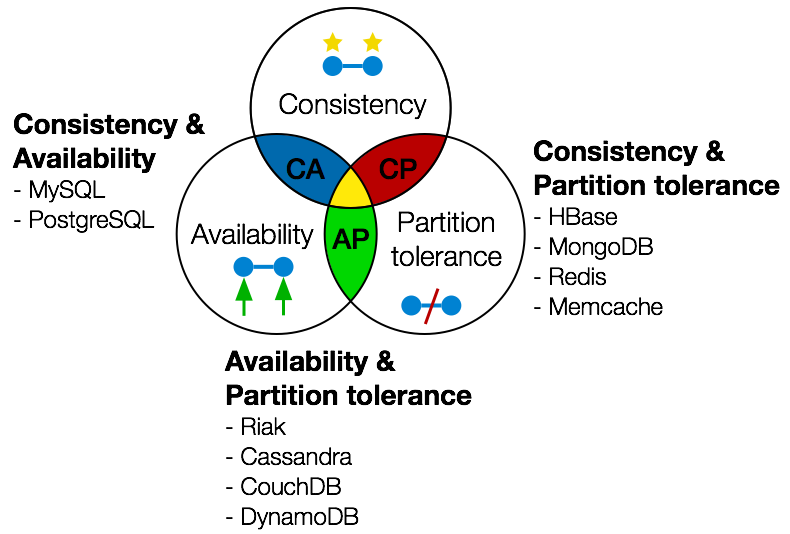
\includegraphics[width=0.7\textwidth]{gfx/CAPTheorem.png}
  \caption{Clasificación de bases de datos mediante el teorema de CAP.}
\end{figure}

\section{Tipos de bases de datos NoSQL}

En esta sección vamos a caracterizar las bases de datos NoSQL según la forma en la que almacenen los datos. Podemos clasificar la mayoría de bases de datos NoSQL en alguna de las siguientes 4 categorías, como se describe en la propia documentación de MongoDB \cite{mongoclassification}.

\begin{itemize}
    \item \texttt{Almacenamiento clave-valor}: Son grandes tablas que almacenan la información en forma de clave-valor. Las bases de datos de este tipo más populares son: RedisDB, Riak y Voldemort.
    \item \texttt{Almacenamiento basado en documentos}: Es este tipo de bases de datos, los datos se almacenan en forma de documentos. El concepto de documento depende de la definición de la base de datos, normalmente son grandes conjuntos de claves-valor codificados o encapsulados como un tipo de documento. En esta sección, Mongo DB es el más popular y más usado, pero existen otros como Couch DB.
    \item \texttt{Almacenamiento basado en grafos}: Estas bases de datos almacenan relaciones en forma de grafos. Algunas de las bases de datos más populares son: Neo4j y FlockDB.
    \item \texttt{Almacenamiento en columnas}: En este tipo de bases de datos, se almacenan columnas en lugar de filas como en el resto de tipos. Está optimizado para grandes volúmenes de datos. Las bases de datos más populares de este tipo son: Cassandra y HBase. 
\end{itemize}

En el artículo \cite{nosqlcomparativas}, puede verse una comparativa entre distintas bases de datos NoSQL sobre lenguaje en el que están escritas, ternologías que utilizan, tipo de base de datos, etc.

\section{Comparativa NoSQL con SGBDR}

En esta sección vamos a realizar una comparativa entre las bases de datos SQL y NoSQL.

En primer lugar, además de las dos diferencias comentadas anteriormente, es de destacar, que las bases de datos NoSQL son libres de esquema, esto es, que no necesitan una planificación antes de empezar a almacenar datos a nivel de relaciones, tablas, etc. Los datos almacenados son independientes entre ellos y pueden ser totalmente distintos. Esto aporta un gran valor en el sentido de adaptabilidad a nuevos cambios.

\subsection{SGBDR}

Vamos a dar algunas características que caracterizan a las bases de datos SGBDR, para comenzar veremos algunos de las características favorables de este tipo de base de datos:

\begin{itemize}
    \item Mayor soporte y herramientas debido a su largo recorrido en el mercado.
    \item Permite combinar diferentes tablas eficientemente para obtener información relacionada.
    \item Los datos siguen una estructura predefinida en los esquemas.
    \item Proporcionan atomicidad en las operaciones y transaccionalidad entre tablas, esto evita que se queden datos inconsistentes si hay un error en cualquier punto de una operación.
\end{itemize}

Por contra:

\begin{itemize}
    \item No son flexibles, en el sentido de que los datos tienen que seguir el esquema definido y tienen que estar correctamente validados.
    \item Incremento del procesamiento con el incremento de la complejidad en las relaciones.
    \item Dificultad para escalar, habitualmente necesitan de ampliación de hardware costoso.
\end{itemize}

\subsection{NoSQL}

Una de las principales características que tendría el conjunto de bases de datos NoSQL, es que proporcionan una manera alternativa de almacenar la información y muy diversa por los tipos que comentamos anteriormente, por tanto, ya nos proporcionan una cierta ventaja de flexibilidad que no tenemos con los sistemas SGBDR tradicionales. Veamos ahora algunas características favorables que poseen las bases de datos NoSQL:

\begin{itemize}
    \item Escalabilidad. En general, tienen buen escalamiento horizontal.
    \item Soporte para modelos flexibles, libres de esquemas, tipos y validaciones.
    \item Optimiazadas para gande volúmenes de datos.
    \item Necesita de pocos recursos para su funcionamiento.
\end{itemize}

Por contra:

\begin{itemize}
    \item No todas garantizas atomicidad y consistencia en los datos.
    \item Falta de estandarización. No existe un estándar para estas bases de datos como si lo hay para las de tipo SQL.
    \item Falta de herramientas de gestión. Muchas de ellas solo son accesibles por consola.
\end{itemize}


\section{Mongo DB}

En esta sección vamos a centrarnos en la base de datos NoSQL más popular hasta el momento, mongo db es una base de datos orientada a documentos y muy usada para técnicas de Big Data.



% NOSQL-MONGO:
    % 1. Historia
    % 2. Características
    % 3. SQL vs NoSQL
    % 4. Ejemplos y usos
    % 5. MongoDb (Note: Como representa los datos y como se consultan)
